\section*{Structure}

The theory part consist of 4 chapters. Chapter 3, 4 and 5 presents the three theoretical theories I have used. And chapter 6 is a constellation of the three chapters and my proposal of a new theoretical lens to look at meaningfulness in a museum context.
\begin{itemize}
    \item Chapter 3: Hybrid place
    \item Chapter 4: Place as a dialogue
    \item Chapter 5: Sense-making
    \item Chapter 6: A new way to design for meaningfulness?
\end{itemize}
\par


\section*{Use of theory}
The use of theory is essential to any academic discipline. Before we embark on to the Theory chapters, it is necessary to go into how theory have been put to use throughout the thesis project. Theory takes researchers beyond observation and interpretation into the realm of shareable knowledge \autocite[p. 126]{beck_examining_2016}. It provides us with the means to structure knowledge, to evaluate and assess it, to construct it, and to share it \autocite[p. 126]{beck_examining_2016}. In a paper examining the practical, everyday theory use in design research, Beck and Stolterman discuss how researchers put theories to work in their written texts, and synthesise six models of "theory use". The models reflect the different ways researchers make use of theory beyond the commonly referenced uses of explanation, generalisation, prediction, and the like. And shows how theory can be used to motivate inquiry, contextualize research, shape research questions and guide methodology and analysis \autocite[p. 134]{beck_examining_2016}. The six models they propose is namely: no theory, theory as the object of study, theory as a contextualising tool, theory as a shaping tool, theory as a methodological tool, and theory as an analytical tool. Theory has primarily been put to use as a contextual and analytical tool in this thesis. 

\begin{figure}[H]
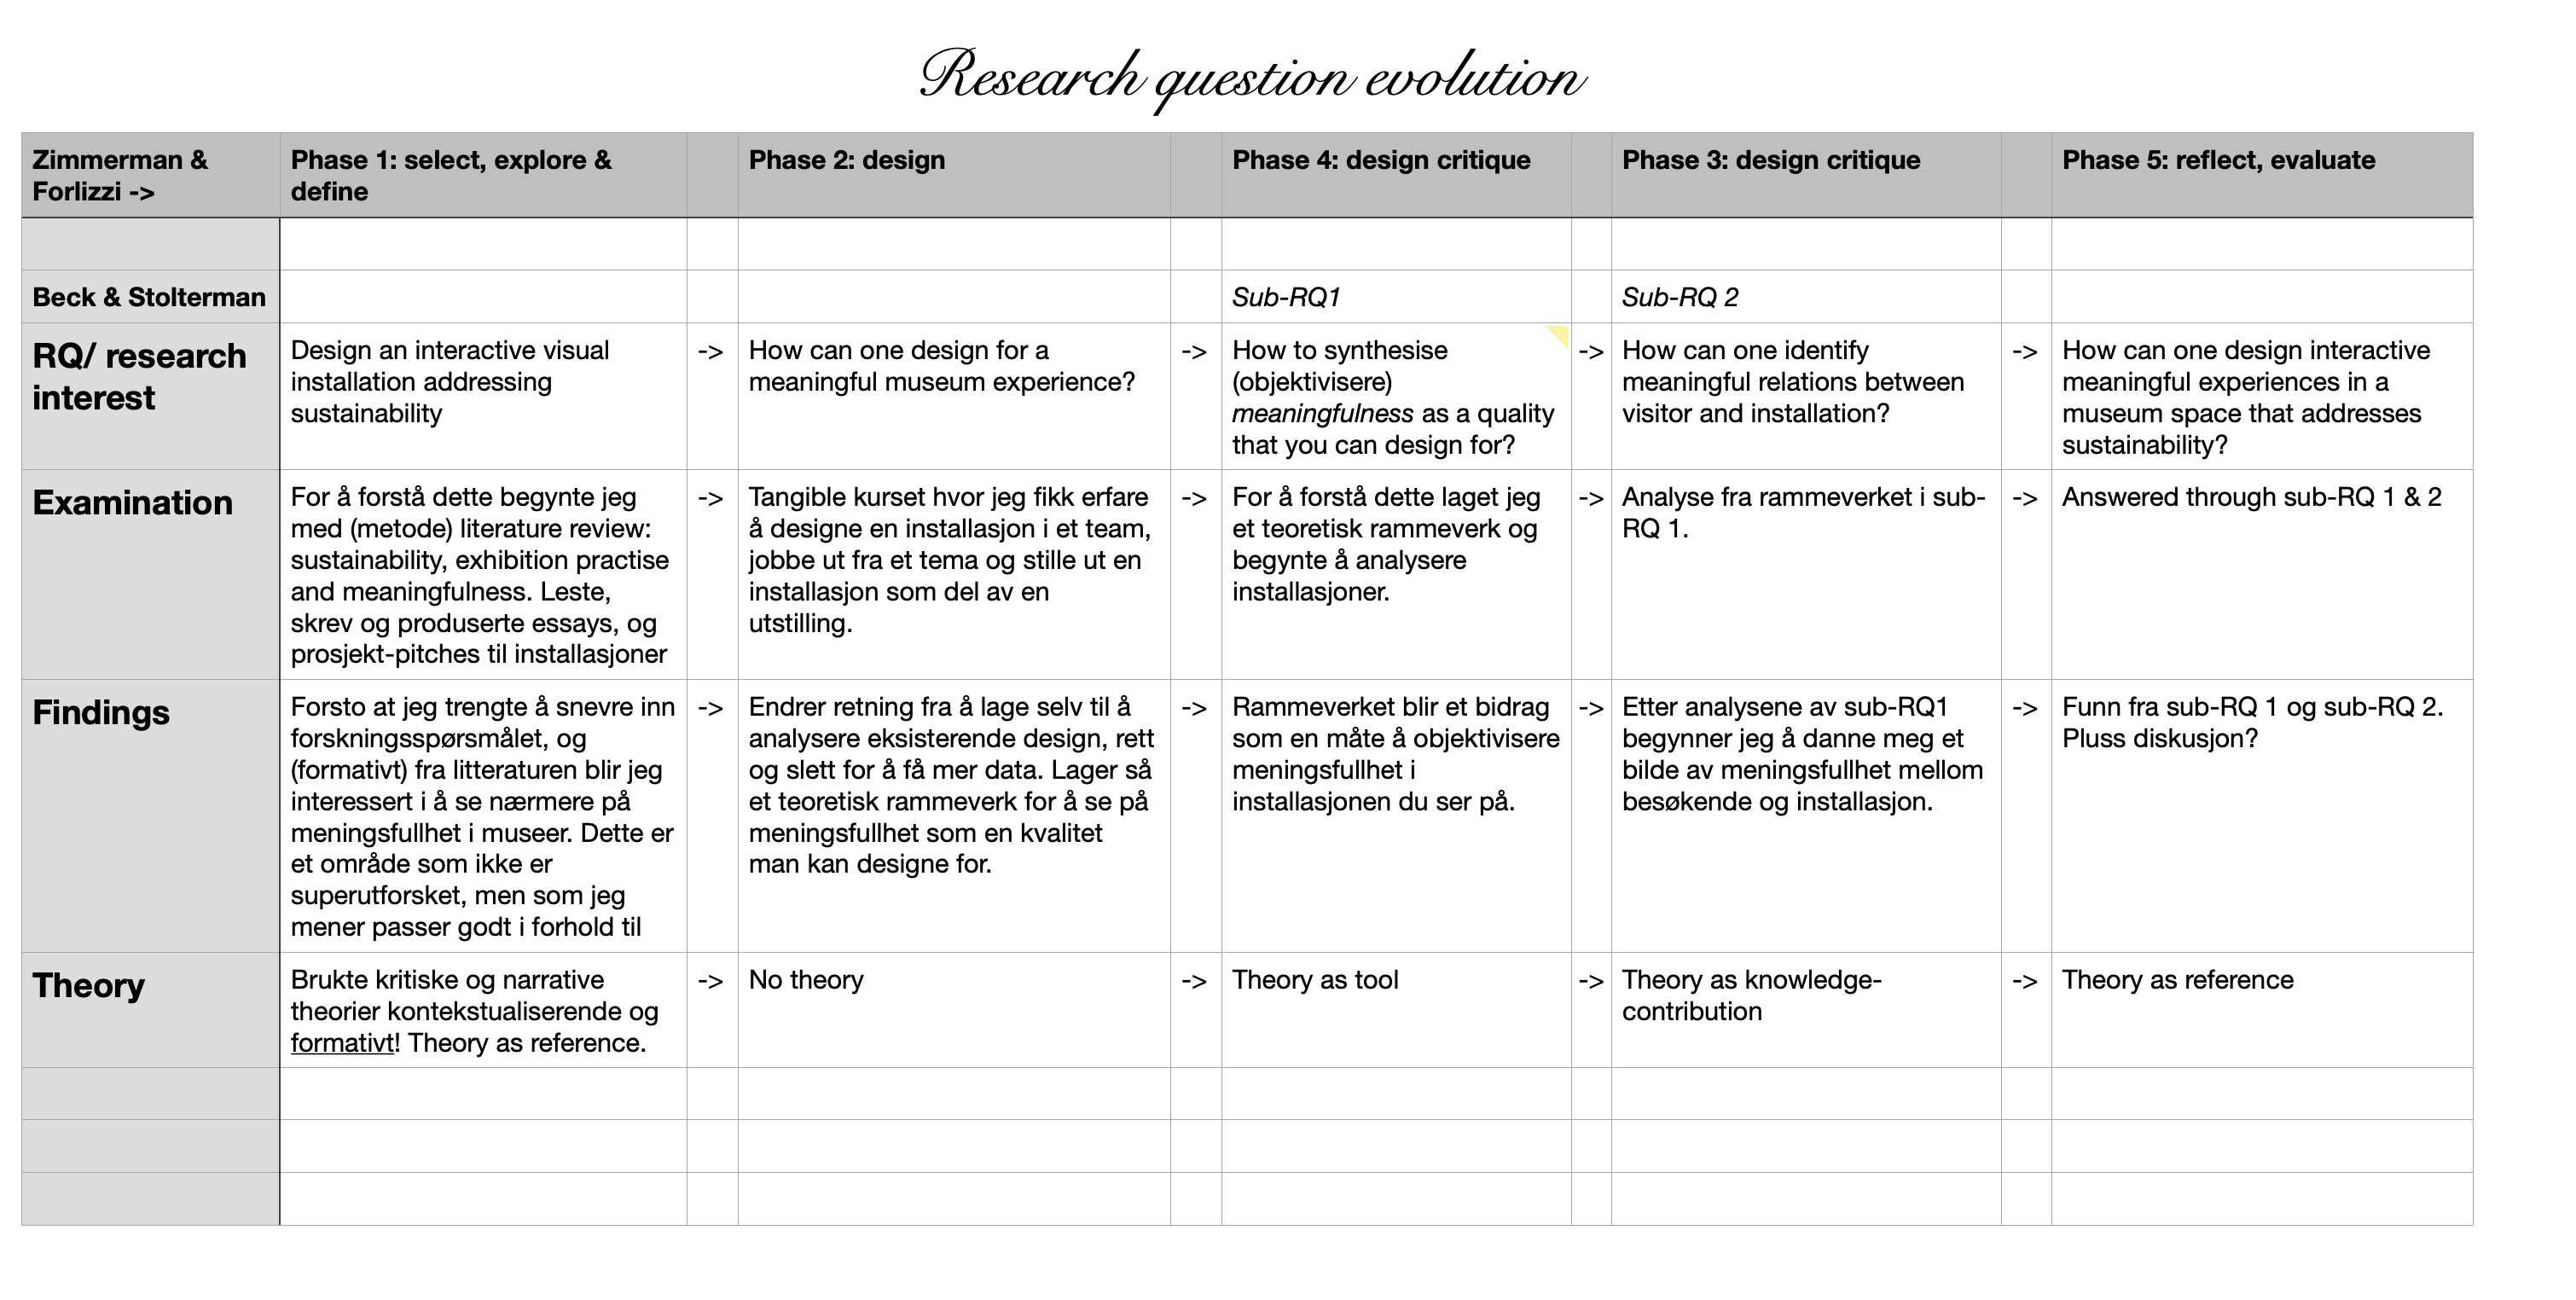
\includegraphics[width=13cm]{pictures/process/rq_evolution.png}
\caption{Research question evolution}
\centering 
\end{figure}



\par \emph{Theory as an object} \par
"When a researcher develops an explanation of how or why some phenomenon occurs, they are engaged in theorizing a \emph{process}" \autocite[p.126]{beck_examining_2016}. The explanation itself becomes a theoretical \emph{object} \autocite[p. 126]{beck_examining_2016}.  


\par \emph{Theory as a tool} \par

Framing theory as a tool implies that a user uses theory for a particular purpose. Theory has been described and defined by many researchers in terms of its utility. It has been framed as a tool for explaining, describing, or predicting phenomena. It has been described in design research as a tool for "binding together" our knowledge of design practise and as a tool for "providing an understanding" of design writ large. \autocite[p. 127]{beck_examining_2016}. Similarly, theory is not necessarily an ideal tool for explaining reality in the same way that an analogy or metaphor might be. THeory, a tool for explaining, predicting, or describing, has structural properties conducive to other purposes as well. \autocite[p. 127]{beck_examining_2016}.


\par \emph{Theory as a reference} \par
Common definitions of reference include: the action of mentioning or alluding to something or the use of information to ascertain something. When theory is used as a reference, it most often appears in the introductory and/or background section of a given wrritten text \autocite[p. 128]{beck_examining_2016}. With this type of of theory use, researchers often reference frameworks and models \emph{instead} of referencing theory per se. Theory as a reference can perform several functions that may appear in concert or individually in a given research paper. For instance, a theory can be used to etablish the basis for a research project, to situate a text within a lineage, to establish the knowledge base of the writer, or to show connection to a community or school of thought. 
\par
(Mieke Bal narrative theories etc is an example of how  have used theory as a reference!)

\par \emph{Theory as a knowledge contribution} \par
Characterising theory as a \emph{knowledge contribution} suggests that it had not existed prior to the researcher's articulation of it. The researchers brought it into being by formulating their results such that they would be understood as a theory, for instance, as a set of constructs and their definitions, as well as a set of propositions about how the construct relate to one another. This formulation of a theory becomes a knowledge object. \autocite[p. 128]{beck_examining_2016}.



